% Options for packages loaded elsewhere
\PassOptionsToPackage{unicode}{hyperref}
\PassOptionsToPackage{hyphens}{url}
\PassOptionsToPackage{dvipsnames,svgnames,x11names}{xcolor}
%
\documentclass[
  letterpaper,
  DIV=11,
  numbers=noendperiod]{scrartcl}

\usepackage{amsmath,amssymb}
\usepackage{iftex}
\ifPDFTeX
  \usepackage[T1]{fontenc}
  \usepackage[utf8]{inputenc}
  \usepackage{textcomp} % provide euro and other symbols
\else % if luatex or xetex
  \usepackage{unicode-math}
  \defaultfontfeatures{Scale=MatchLowercase}
  \defaultfontfeatures[\rmfamily]{Ligatures=TeX,Scale=1}
\fi
\usepackage{lmodern}
\ifPDFTeX\else  
    % xetex/luatex font selection
\fi
% Use upquote if available, for straight quotes in verbatim environments
\IfFileExists{upquote.sty}{\usepackage{upquote}}{}
\IfFileExists{microtype.sty}{% use microtype if available
  \usepackage[]{microtype}
  \UseMicrotypeSet[protrusion]{basicmath} % disable protrusion for tt fonts
}{}
\makeatletter
\@ifundefined{KOMAClassName}{% if non-KOMA class
  \IfFileExists{parskip.sty}{%
    \usepackage{parskip}
  }{% else
    \setlength{\parindent}{0pt}
    \setlength{\parskip}{6pt plus 2pt minus 1pt}}
}{% if KOMA class
  \KOMAoptions{parskip=half}}
\makeatother
\usepackage{xcolor}
\usepackage[left=1in,right=1in,top=1in,bottom=1in]{geometry}
\setlength{\emergencystretch}{3em} % prevent overfull lines
\setcounter{secnumdepth}{-\maxdimen} % remove section numbering
% Make \paragraph and \subparagraph free-standing
\ifx\paragraph\undefined\else
  \let\oldparagraph\paragraph
  \renewcommand{\paragraph}[1]{\oldparagraph{#1}\mbox{}}
\fi
\ifx\subparagraph\undefined\else
  \let\oldsubparagraph\subparagraph
  \renewcommand{\subparagraph}[1]{\oldsubparagraph{#1}\mbox{}}
\fi


\providecommand{\tightlist}{%
  \setlength{\itemsep}{0pt}\setlength{\parskip}{0pt}}\usepackage{longtable,booktabs,array}
\usepackage{calc} % for calculating minipage widths
% Correct order of tables after \paragraph or \subparagraph
\usepackage{etoolbox}
\makeatletter
\patchcmd\longtable{\par}{\if@noskipsec\mbox{}\fi\par}{}{}
\makeatother
% Allow footnotes in longtable head/foot
\IfFileExists{footnotehyper.sty}{\usepackage{footnotehyper}}{\usepackage{footnote}}
\makesavenoteenv{longtable}
\usepackage{graphicx}
\makeatletter
\def\maxwidth{\ifdim\Gin@nat@width>\linewidth\linewidth\else\Gin@nat@width\fi}
\def\maxheight{\ifdim\Gin@nat@height>\textheight\textheight\else\Gin@nat@height\fi}
\makeatother
% Scale images if necessary, so that they will not overflow the page
% margins by default, and it is still possible to overwrite the defaults
% using explicit options in \includegraphics[width, height, ...]{}
\setkeys{Gin}{width=\maxwidth,height=\maxheight,keepaspectratio}
% Set default figure placement to htbp
\makeatletter
\def\fps@figure{htbp}
\makeatother

\usepackage{fvextra}
\DefineVerbatimEnvironment{Highlighting}{Verbatim}{breaklines,commandchars=\\\{\}}
\DefineVerbatimEnvironment{OutputCode}{Verbatim}{breaklines,commandchars=\\\{\}}
\KOMAoption{captions}{tableheading}
\makeatletter
\makeatother
\makeatletter
\makeatother
\makeatletter
\@ifpackageloaded{caption}{}{\usepackage{caption}}
\AtBeginDocument{%
\ifdefined\contentsname
  \renewcommand*\contentsname{Table of contents}
\else
  \newcommand\contentsname{Table of contents}
\fi
\ifdefined\listfigurename
  \renewcommand*\listfigurename{List of Figures}
\else
  \newcommand\listfigurename{List of Figures}
\fi
\ifdefined\listtablename
  \renewcommand*\listtablename{List of Tables}
\else
  \newcommand\listtablename{List of Tables}
\fi
\ifdefined\figurename
  \renewcommand*\figurename{Figure}
\else
  \newcommand\figurename{Figure}
\fi
\ifdefined\tablename
  \renewcommand*\tablename{Table}
\else
  \newcommand\tablename{Table}
\fi
}
\@ifpackageloaded{float}{}{\usepackage{float}}
\floatstyle{ruled}
\@ifundefined{c@chapter}{\newfloat{codelisting}{h}{lop}}{\newfloat{codelisting}{h}{lop}[chapter]}
\floatname{codelisting}{Listing}
\newcommand*\listoflistings{\listof{codelisting}{List of Listings}}
\makeatother
\makeatletter
\@ifpackageloaded{caption}{}{\usepackage{caption}}
\@ifpackageloaded{subcaption}{}{\usepackage{subcaption}}
\makeatother
\makeatletter
\@ifpackageloaded{tcolorbox}{}{\usepackage[skins,breakable]{tcolorbox}}
\makeatother
\makeatletter
\@ifundefined{shadecolor}{\definecolor{shadecolor}{rgb}{.97, .97, .97}}
\makeatother
\makeatletter
\makeatother
\makeatletter
\makeatother
\ifLuaTeX
  \usepackage{selnolig}  % disable illegal ligatures
\fi
\IfFileExists{bookmark.sty}{\usepackage{bookmark}}{\usepackage{hyperref}}
\IfFileExists{xurl.sty}{\usepackage{xurl}}{} % add URL line breaks if available
\urlstyle{same} % disable monospaced font for URLs
\hypersetup{
  pdftitle={SDS 291 Final Project: Topic and Data Selection},
  pdfauthor={Miya Dang, Mia Tran, Alua Birgebayeva},
  colorlinks=true,
  linkcolor={blue},
  filecolor={Maroon},
  citecolor={Blue},
  urlcolor={Blue},
  pdfcreator={LaTeX via pandoc}}

\title{SDS 291 Final Project: Topic and Data Selection}
\author{Miya Dang, Mia Tran, Alua Birgebayeva}
\date{2025-04-28}

\begin{document}
\maketitle
\ifdefined\Shaded\renewenvironment{Shaded}{\begin{tcolorbox}[boxrule=0pt, frame hidden, sharp corners, borderline west={3pt}{0pt}{shadecolor}, enhanced, interior hidden, breakable]}{\end{tcolorbox}}\fi

\hypertarget{data}{%
\section{Data}\label{data}}

The dataset we are using for the final project is the Heart Failure
Clinical Records Dataset, originally sourced from the UCI Machine
Learning Repository
(\url{https://archive.ics.uci.edu/dataset/519/heart+failure+clinical+records}).
It contains the medical records of 299 patients who experienced heart
failure, collected during their follow-up period. Each observation is a
patient profile, with 13 variables measuring their clinical records such
as blood test results, whether or not they have diabetes or
hypertension, as well as their age and sex.

\hypertarget{research-questionpurpose}{%
\section{Research Question/Purpose}\label{research-questionpurpose}}

Our project aims to answer the following research question:
\textbf{Which clinical characteristics are most predictive of death
among patients with heart failure?}

We will identify important predictors that may offer insights into
patient outcomes after heart failure. Then, using multiple logistic
regression, we will model the probability of death during the follow-up
period based on clinical data.

\hypertarget{response-variable}{%
\section{Response Variable}\label{response-variable}}

Our response variable is DEATH\_EVENT, a binary categorical variable
with 2 levels:

\begin{itemize}
\item
  0 = Patient survived during the follow-up period (considered
  ``failure'' when modelling).
\item
  1 = Patient died during the follow-up period (considered ``success''
  when modelling).
\end{itemize}

\hypertarget{explanatory-variables}{%
\section{Explanatory Variables}\label{explanatory-variables}}

We plan to include all 12 variables other than DEATH\_EVENT as
explanatory variables to include in the richest possible model .

\begin{longtable}[]{@{}
  >{\raggedright\arraybackslash}p{(\columnwidth - 6\tabcolsep) * \real{0.2500}}
  >{\raggedright\arraybackslash}p{(\columnwidth - 6\tabcolsep) * \real{0.2500}}
  >{\raggedright\arraybackslash}p{(\columnwidth - 6\tabcolsep) * \real{0.2500}}
  >{\raggedright\arraybackslash}p{(\columnwidth - 6\tabcolsep) * \real{0.2500}}@{}}
\toprule\noalign{}
\begin{minipage}[b]{\linewidth}\raggedright
Variable
\end{minipage} & \begin{minipage}[b]{\linewidth}\raggedright
Type
\end{minipage} & \begin{minipage}[b]{\linewidth}\raggedright
Description
\end{minipage} & \begin{minipage}[b]{\linewidth}\raggedright
Units/Levels
\end{minipage} \\
\midrule\noalign{}
\endhead
\bottomrule\noalign{}
\endlastfoot
\textbf{age} & Numeric & Age of the patient & Years (40--95) \\
\textbf{anaemia} & Categorical & Presence of anemia (decrease of red
blood cells or hemoglobin) & 0 = No, 1 = Yes \\
\textbf{creatinine\_phosphokinase} & Numeric & Level of CPK enzyme in
blood (indicator of muscle damage) & mcg/L (23--7861) \\
\textbf{diabetes} & Categorical & Presence of diabetes & 0 = No, 1 =
Yes \\
\textbf{ejection\_fraction} & Numeric & Percentage of blood leaving the
heart at each contraction & \% (14--80) \\
\textbf{high\_blood\_pressure} & Categorical & Presence of hypertension
(high blood pressure) & 0 = No, 1 = Yes \\
\textbf{platelets} & Numeric & Amount of platelets in the blood &
kiloplatelets/mL (\textasciitilde25,000--850,000) \\
\textbf{serum\_creatinine} & Numeric & Level of serum creatinine in
blood (kidney function indicator) & mg/dL (0.5--9.4) \\
\textbf{serum\_sodium} & Numeric & Level of serum sodium in blood &
mEq/L (113--148) \\
\textbf{sex} & Categorical & Gender of patient & 0 = Woman, 1 = Man \\
\textbf{smoking} & Categorical & Smoking status of patient & 0 = No, 1 =
Yes \\
\textbf{time} & Numeric & Length of follow-up period & Days (4--285) \\
\end{longtable}

\hypertarget{exploratory-visualizations}{%
\section{Exploratory Visualizations}\label{exploratory-visualizations}}

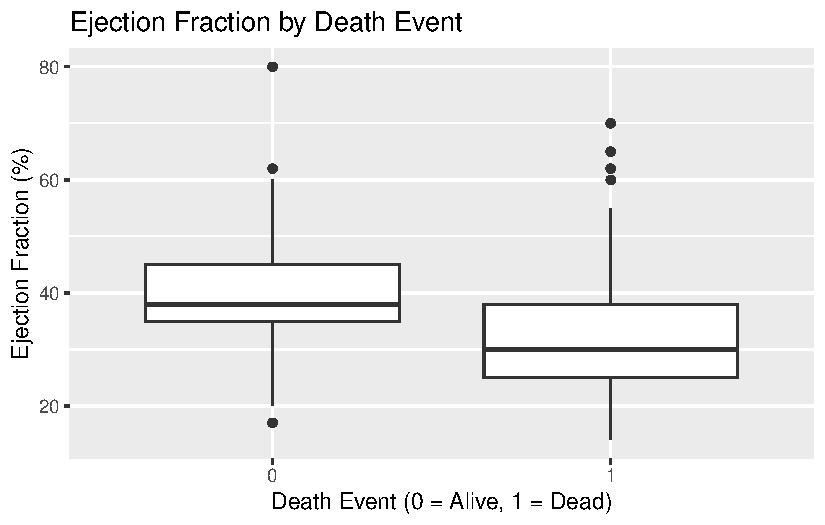
\includegraphics{SDS-291-final-project_files/figure-pdf/unnamed-chunk-2-1.pdf}

The first boxplot shows that ejection fraction was generally lower among
patients who died compared to those who survived, suggesting reduced
heart pumping function as a key predictor of mortality.

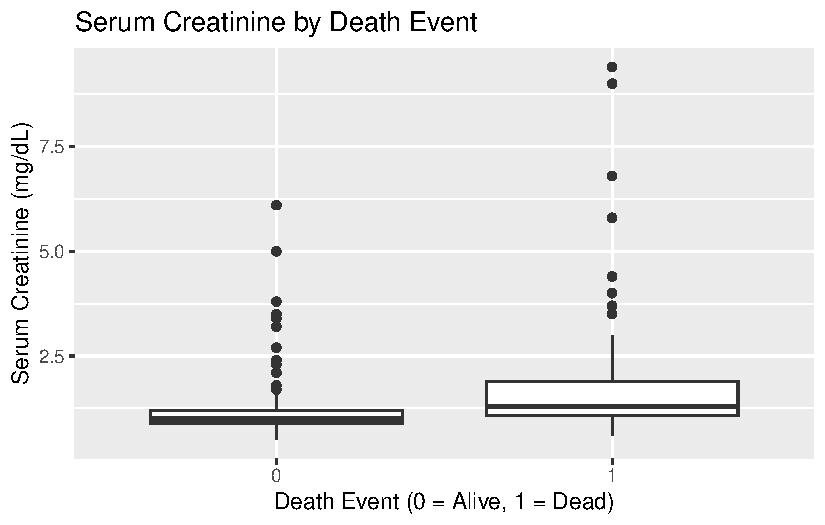
\includegraphics{SDS-291-final-project_files/figure-pdf/unnamed-chunk-3-1.pdf}

The second boxplot shows that serum creatinine levels were higher among
patients who died, indicating that impaired kidney function is
associated with worse outcomes in heart failure patients.



\end{document}
